\documentclass[oneside]{book}
\usepackage{amsmath, amsthm, amssymb, amsfonts}
\usepackage{thmtools}
\usepackage{graphicx}
\usepackage{setspace}
\usepackage{geometry}
\usepackage{float}
\usepackage{hyperref}
\usepackage[utf8]{inputenc}
\usepackage[english]{babel}
\usepackage{framed}
\usepackage[dvipsnames]{xcolor}
\usepackage{environ}
\usepackage{tcolorbox}
\tcbuselibrary{theorems,skins,breakable}

\setstretch{1.2}
\geometry{
    textheight=9in,
    textwidth=5.5in,
    top=1in,
    headheight=12pt,
    headsep=25pt,
    footskip=30pt
}

% Variables
\def\notetitle{Calculus I}
\def\noteauthor{
    \textbf{T.A. Hazem Hossam} \\ 
    {\LaTeX} by Joe\\
    University}
\def\notedate{Semester}

% The theorem system and user-defined commands
\usepackage{amsfonts, amsmath, amssymb, physics}
\usepackage{mathrsfs}

% Theorem System
% The following boxes are provided:
%   Definition:     \defn 
%   Theorem:        \thm 
%   Lemma:          \lem
%   Corollary:      \cor
%   Proposition:    \prop   
%   Claim:          \clm
%   Fact:           \fact
%   Proof:          \pf
%   Example:        \ex
%   Remark:         \rmk (sentence), \rmkb (block)
% Suffix
%   r:              Allow Theorem/Definition to be referenced, e.g. thmr
%   p:              Add a short proof block for Lemma, Corollary, Proposition or Claim, e.g. lemp
%                   For theorems, use \pf for proof blocks
% solution:           \soln
% Definition
\newtcbtheorem[number within=section]{mydefinition}{Definition}
{
    enhanced,
    frame hidden,
    titlerule=0mm,
    toptitle=1mm,
    bottomtitle=1mm,
    fonttitle=\bfseries\large,
    coltitle=black,
    colbacktitle=green!20!white,
    colback=green!10!white,
}{defn}

\NewDocumentCommand{\defn}{m+m}{
    \begin{mydefinition}{#1}{}
        #2
    \end{mydefinition}
}

\NewDocumentCommand{\defnr}{mm+m}{
    \begin{mydefinition}{#1}{#2}
        #3
    \end{mydefinition}
}

% Theorem
\newtcbtheorem[use counter from=mydefinition]{mytheorem}{Theorem}
{
    enhanced,
    frame hidden,
    titlerule=0mm,
    toptitle=1mm,
    bottomtitle=1mm,
    fonttitle=\bfseries\large,
    coltitle=black,
    colbacktitle=cyan!20!white,
    colback=cyan!10!white,
}{thm}

\NewDocumentCommand{\thm}{m+m}{
    \begin{mytheorem}{#1}{}
        #2
    \end{mytheorem}
}

\NewDocumentCommand{\thmr}{mm+m}{
    \begin{mytheorem}{#1}{#2}
        #3
    \end{mytheorem}
}

% Lemma
\newtcbtheorem[use counter from=mydefinition]{mylemma}{Lemma}
{
    enhanced,
    frame hidden,
    titlerule=0mm,
    toptitle=1mm,
    bottomtitle=1mm,
    fonttitle=\bfseries\large,
    coltitle=black,
    colbacktitle=violet!20!white,
    colback=violet!10!white,
}{lem}

\NewDocumentCommand{\lem}{m+m}{
    \begin{mylemma}{#1}{}
        #2
    \end{mylemma}
}

\newenvironment{lempf}{
	{\noindent{\it \textbf{Proof for Lemma}}}
	\tcolorbox[blanker,breakable,left=5mm,parbox=false,
    before upper={\parindent15pt},
    after skip=10pt,
	borderline west={1mm}{0pt}{violet!20!white}]
}{
    \textcolor{violet!20!white}{\hbox{}\nobreak\hfill$\blacksquare$} 
    \endtcolorbox
}

\NewDocumentCommand{\lemp}{m+m+m}{
    \begin{mylemma}{#1}{}
        #2
    \end{mylemma}

    \begin{lempf}
        #3
    \end{lempf}
}

% Corollary
\newtcbtheorem[use counter from=mydefinition]{mycorollary}{Corollary}
{
    enhanced,
    frame hidden,
    titlerule=0mm,
    toptitle=1mm,
    bottomtitle=1mm,
    fonttitle=\bfseries\large,
    coltitle=black,
    colbacktitle=orange!20!white,
    colback=orange!10!white,
}{cor}

\NewDocumentCommand{\cor}{+m}{
    \begin{mycorollary}{}{}
        #1
    \end{mycorollary}
}

\newenvironment{corpf}{
	{\noindent{\it \textbf{Proof for Corollary.}}}
	\tcolorbox[blanker,breakable,left=5mm,parbox=false,
    before upper={\parindent15pt},
    after skip=10pt,
	borderline west={1mm}{0pt}{orange!20!white}]
}{
    \textcolor{orange!20!white}{\hbox{}\nobreak\hfill$\blacksquare$} 
    \endtcolorbox
}

\NewDocumentCommand{\corp}{m+m+m}{
    \begin{mycorollary}{}{}
        #1
    \end{mycorollary}

    \begin{corpf}
        #2
    \end{corpf}
}

% Proposition
\newtcbtheorem[use counter from=mydefinition]{myproposition}{Proposition}
{
    enhanced,
    frame hidden,
    titlerule=0mm,
    toptitle=1mm,
    bottomtitle=1mm,
    fonttitle=\bfseries\large,
    coltitle=black,
    colbacktitle=yellow!30!white,
    colback=yellow!20!white,
}{prop}

\NewDocumentCommand{\prop}{+m}{
    \begin{myproposition}{}{}
        #1
    \end{myproposition}
}

\newenvironment{proppf}{
	{\noindent{\it \textbf{Proof for Proposition.}}}
	\tcolorbox[blanker,breakable,left=5mm,parbox=false,
    before upper={\parindent15pt},
    after skip=10pt,
	borderline west={1mm}{0pt}{yellow!30!white}]
}{
    \textcolor{yellow!30!white}{\hbox{}\nobreak\hfill$\blacksquare$} 
    \endtcolorbox
}

\NewDocumentCommand{\propp}{+m+m}{
    \begin{myproposition}{}{}
        #1
    \end{myproposition}

    \begin{proppf}
        #2
    \end{proppf}
}

% Claim
\newtcbtheorem[use counter from=mydefinition]{myclaim}{Claim}
{
    enhanced,
    frame hidden,
    titlerule=0mm,
    toptitle=1mm,
    bottomtitle=1mm,
    fonttitle=\bfseries\large,
    coltitle=black,
    colbacktitle=pink!30!white,
    colback=pink!20!white,
}{clm}


\NewDocumentCommand{\clm}{m+m}{
    \begin{myclaim*}{#1}{}
        #2
    \end{myclaim*}
}

\newenvironment{clmpf}{
	{\noindent{\it \textbf{Proof for Claim.}}}
	\tcolorbox[blanker,breakable,left=5mm,parbox=false,
    before upper={\parindent15pt},
    after skip=10pt,
	borderline west={1mm}{0pt}{pink!30!white}]
}{
    \textcolor{pink!30!white}{\hbox{}\nobreak\hfill$\blacksquare$} 
    \endtcolorbox
}

\NewDocumentCommand{\clmp}{m+m+m}{
    \begin{myclaim*}{#1}{}
        #2
    \end{myclaim*}

    \begin{clmpf}
        #3
    \end{clmpf}
}

% Fact
\newtcbtheorem{myobj}{Objective}
{
    enhanced,
    frame hidden,
    titlerule=0mm,
    toptitle=1mm,
    bottomtitle=1mm,
    fonttitle=\bfseries\large,
    coltitle=black,
    colbacktitle=white!20!white,
    colback=gray!10!white,
}{obk}

\NewDocumentCommand{\obj}{+m}{
    \begin{myobj*}{}{}
        #1
    \end{myobj*}
}


% Proof
\NewDocumentCommand{\pf}{+m}{
    \begin{proof}
        [\noindent\textbf{Proof.}]
        #1
    \end{proof}
}


% Solution
\NewDocumentCommand{\soln}{+m}{
    \begin{proof}
        [\noindent\textbf{Solution.}]
        #1
    \end{proof}
}

% Example
\newenvironment{example}{%
    \par
    \vspace{5pt}
	\begin{minipage}{\textwidth}
		\noindent\textbf{Example.}
		\tcolorbox[blanker,breakable,left=5mm,parbox=false,
	    before upper={\parindent15pt},
	    after skip=10pt,
		borderline west={1mm}{0pt}{cyan!10!white}]
}{%
		\endtcolorbox
	\end{minipage}
    \vspace{5pt}
}

\NewDocumentCommand{\ex}{+m}{
    \begin{example}
        #1
    \end{example}
}


% Remark
\NewDocumentCommand{\rmk}{+m}{
    {\it \color{blue!50!white}#1}
}

\newenvironment{remark}{
    \par
    \vspace{5pt}
    \begin{minipage}{\textwidth}
        {\par\noindent{\textbf{Remark.}}}
        \tcolorbox[blanker,breakable,left=5mm,
        before skip=10pt,after skip=10pt,
        borderline west={1mm}{0pt}{cyan!10!white}]
}{
        \endtcolorbox
    \end{minipage}
    \vspace{5pt}
}

\NewDocumentCommand{\rmkb}{+m}{
    \begin{remark}
        #1
    \end{remark}
}


\newcommand{\lcm}{\operatorname{lcm}}



% ------------------------------------------------------------------------------

\begin{document}
\title{\textbf{
    \LARGE{\notetitle} \vspace*{10\baselineskip}}
    }
\author{\noteauthor}
\date{\notedate}

\maketitle
\newpage

\tableofcontents
\newpage

% ------------------------------------------------------------------------------
\chapter{Gamma Functions}
\obj{
    \begin{itemize}
        \item Definition of gamma function
        \item understand uses and applications
    \end{itemize}
}
\section{Definitions}
Gamma function denoted by $\Gamma{(x)}$. Also known as generalized factorial function. Gamma has several equivalent definitions.
\defn{Euler Representation}{
    \begin{equation}
        \label{EulerRepresentation}
        \Gamma{(x)} = \lim_{n \to \infty} \frac{n! \, n^x}{x (x+1) (x+2) \dots (x+n-1) (x+n)}
    \end{equation}
}

\rmk{
    Limit exist if $x \neq 0 \text{ or negative number} $.
}

\defn{Integral Representation}{
    \begin{equation}
        \label{IntegralRepresentation}
        \Gamma{(x)} =\int_0^\infty e^{-t} t^{x-1} \, dt \quad,x>0
    \end{equation}
}

\rmk{
Integral ($\ref{IntegralRepresentation}$) is improper integral due to the infinite upper limit of integration and $t^{x-1}$ at $t=0$ when $0<x<1$\\
}


Let's take a look on some important properties (using ($\ref{EulerRepresentation}$) and ($\ref{IntegralRepresentation}$))\\

\begin{itemize}
    \item What is the value of $\Gamma{(1)}$ ?
          \begin{align*}
              \Gamma{(1)} & = \lim_{n \to \infty} \frac{n! \, n}{1.2.3\dots(n+1)} \\
                          & = \lim_{n \to \infty} \frac{n! \, n}{(n+1)!}          \\
                          & = \lim_{n \to \infty} \frac{n}{n+1} = 1               \\
          \end{align*}
          Or using the integral representation
          \begin{align*}
              \Gamma{(1)} & = \int_0^\infty e^{-t} t^0 dt \\
                          & = 1                           \\
          \end{align*}
    \item We will deduce an important formula
          \begin{align*}
              \Gamma{(x+1)} & = \lim_{n \to \infty} \frac{n! \, n^{x+1}}{(x+1)(x+2)\dots (x+n)(x+n+1)} \color{red} \times \frac{x}{x}         \\
                            & = \lim_{n \to \infty} \frac{n! \, n^x}{ x(x+1)(x+2)\dots (x+n)} \times \lim_{n \to \infty} \frac{n \, x}{x+n+1} \\
                            & = \Gamma{(x)} x
          \end{align*}

Or from integral representation
          \begin{align*}
              \Gamma{(x+1)} & =\int_0^\infty e^{-t} t^x \, dt \quad \color{red}\text{By parts}            \\
                            & = \left[-e^{-t} t^x \right]_0^\infty + \int_0^\infty xe^{-t} t^{x-1}  \, dt \\
                            & = x \int_0^\infty e^{-t} t^{x-1}  \, dt                                     \\
                            & = x \Gamma{(x)}
          \end{align*}
          Hence, An important formula called Recurrence formula
          \begin{equation}
              \label{Recurrenceformula}
              \boxed{\Gamma{(x+1)} = x \Gamma{(x)}}
          \end{equation}
          \rmkb{
            If $x$ is integer $\Gamma{(x+1)} = x! $ or it has another notation by Gauss $\prod(x) = x!$
            }
    \end{itemize}
\ex{
    \begin{itemize}
        \item   $\Gamma{(5)} = 4!$
        \item  $\Gamma{(\frac{3}{2})} = \frac{1}{2} \Gamma{(\frac{1}{2})}$
    \end{itemize}
    }

    Recurrence formula ($\ref{Recurrenceformula}$) can be written as\\
    $$\Gamma{(x)} = \frac{\Gamma{(x+1)}}{x}$$
   \rmkb{
       If $x$ is negative or $ = 0 \quad \Rightarrow \Gamma{(x)}$ divergent
          $$\left|\Gamma{(n)}\right| = \infty ,\quad n \leq 0$$
       }
       \ex{
        \begin{itemize}
            \item $\Gamma{(0)} = \frac{\Gamma{(1)}}{0} = \infty$
            \item $\Gamma{(-1)} = -\infty$
            \item  $\Gamma{(-2)} = \infty$
            \item $\vdots$
        \end{itemize}
        }

    \section{Weierstrass' infinite product}
\defn{Weierstrass' infinite product}{
\begin{equation}
    \label{Weierstrass}
    \frac{1}{\Gamma{(x)}} = x e^{\gamma x} \prod_{n=1}^{\infty} \left(1+ \frac{x}{n} \right) e^{-\frac{x}{n}}
\end{equation}
Where $\gamma$ : Euler-Mascheroni constant
$$\gamma = \lim_{n \to \infty} \left( \sum_{k=1}^{n} \frac{1}{k} -\ln(n) \right) \approx 0.577215 $$
}    


\pf{
    We start with reciprical of Euler representation
\begin{align*}
    \frac{1}{\Gamma{(x)}} &= \lim_{n \to \infty} \frac{x(x+1)(x+2)\dots(x+n)}{n! \, n^x} \\
                          &= x \lim_{n \to \infty} n^{-x} \left( \frac{x+1}{1} \times \frac{x+2}{2} \times \frac{x+3}{3} \dots \frac{x+n}{n} \right) \\
                          &= x \lim_{n \to \infty} e^{-x \ln(n)} \prod_{k=1}^{n} \left(1+\frac{x}{k}\right) \tag{I}
\end{align*}

And obviously, 
\begin{equation}
    \tag{II}
    e^{x \sum_{k=1}^{n} \frac{1}{k}} = \prod_{k=1}^{n} e^{\frac{x}{k}}
\end{equation}
Multiply L.H.S of (II) by (I)

\begingroup
\allowdisplaybreaks
\begin{align*}
    \frac{e^ {x \sum \frac{1}{k}}}{\Gamma{(x)}} &= x \lim_{n \to \infty} e^{-x \ln(n)} \left[ \prod_{k=1}^{n} (1+ \frac{x}{k}) \right] \times e^{x \sum \frac{1}{k}}\\
                                             &= x \lim_{n \to \infty}  \exp \left( x (\sum_{k=1}^{n} \frac{1}{k} - \ln(n) ) \right)  \prod_{k=1}^{n} (1+ \frac{x}{k}) \\
                                          \frac{1}{\Gamma{(x)}}   &= x \lim_{n \to \infty} \exp \left( x (\sum_{k=1}^{n} \frac{1}{k} - \ln(n) ) \right)  \prod_{k=1}^{n} (1+ \frac{x}{k}) \prod_{k=1}^{n}e^{-\frac{x}{k}}\\
                                          &= x \lim_{n \to \infty} \exp \left( x (\sum_{k=1}^{n} \frac{1}{k} - \ln(n) ) \right) \times \lim_{n \to \infty} \prod_{k=1}^{n} \left( 1+ \frac{x}{k}\right) e^{-\frac{x}{k}}\\
                                          &= xe^{\gamma x} \times \prod_{k=1}^{\infty}(1+\frac{x}{k})e^{-\frac{x}{k}}
\end{align*}
\endgroup
}

\newpage


\soln{
sss
}

\thmr{Theorem Name}{mybigthm}{
    A theorem.
}

\lem{Lemma Name}{
    A lemma.
}

\obj{
    A fact.
}

\cor{
    A corollary.
}

\prop{
    A proposition.
}

\clmp{}{
    A claim.
}{
    A reference to Theorem~\ref{thm:mybigthm}
}

\pf{
    Veniam velit incididunt deserunt est proident consectetur non velit ipsum voluptate nulla quis. Ea ullamco consequat non ad amet cupidatat cupidatat aliquip tempor sint ea nisi elit dolore dolore. 

    Laboris labore magna dolore eiusmod ea ex et eiusmod laboris. Et aliquip cupidatat reprehenderit id officia pariatur. 
}

\ex{
    Nostrud esse occaecat Lorem dolore laborum exercitation adipisicing eu sint sunt et. Excepteur voluptate consectetur qui ex amet esse sunt ut nostrud qui proident non. Ipsum nostrud ut elit dolor. Incididunt voluptate esse et est labore cillum proident duis.
}

\rmk{
    Some remark.
}

\rmkb{
    Some more remark.
}

\section{Pictures}

\begin{figure}[H]
    \center
    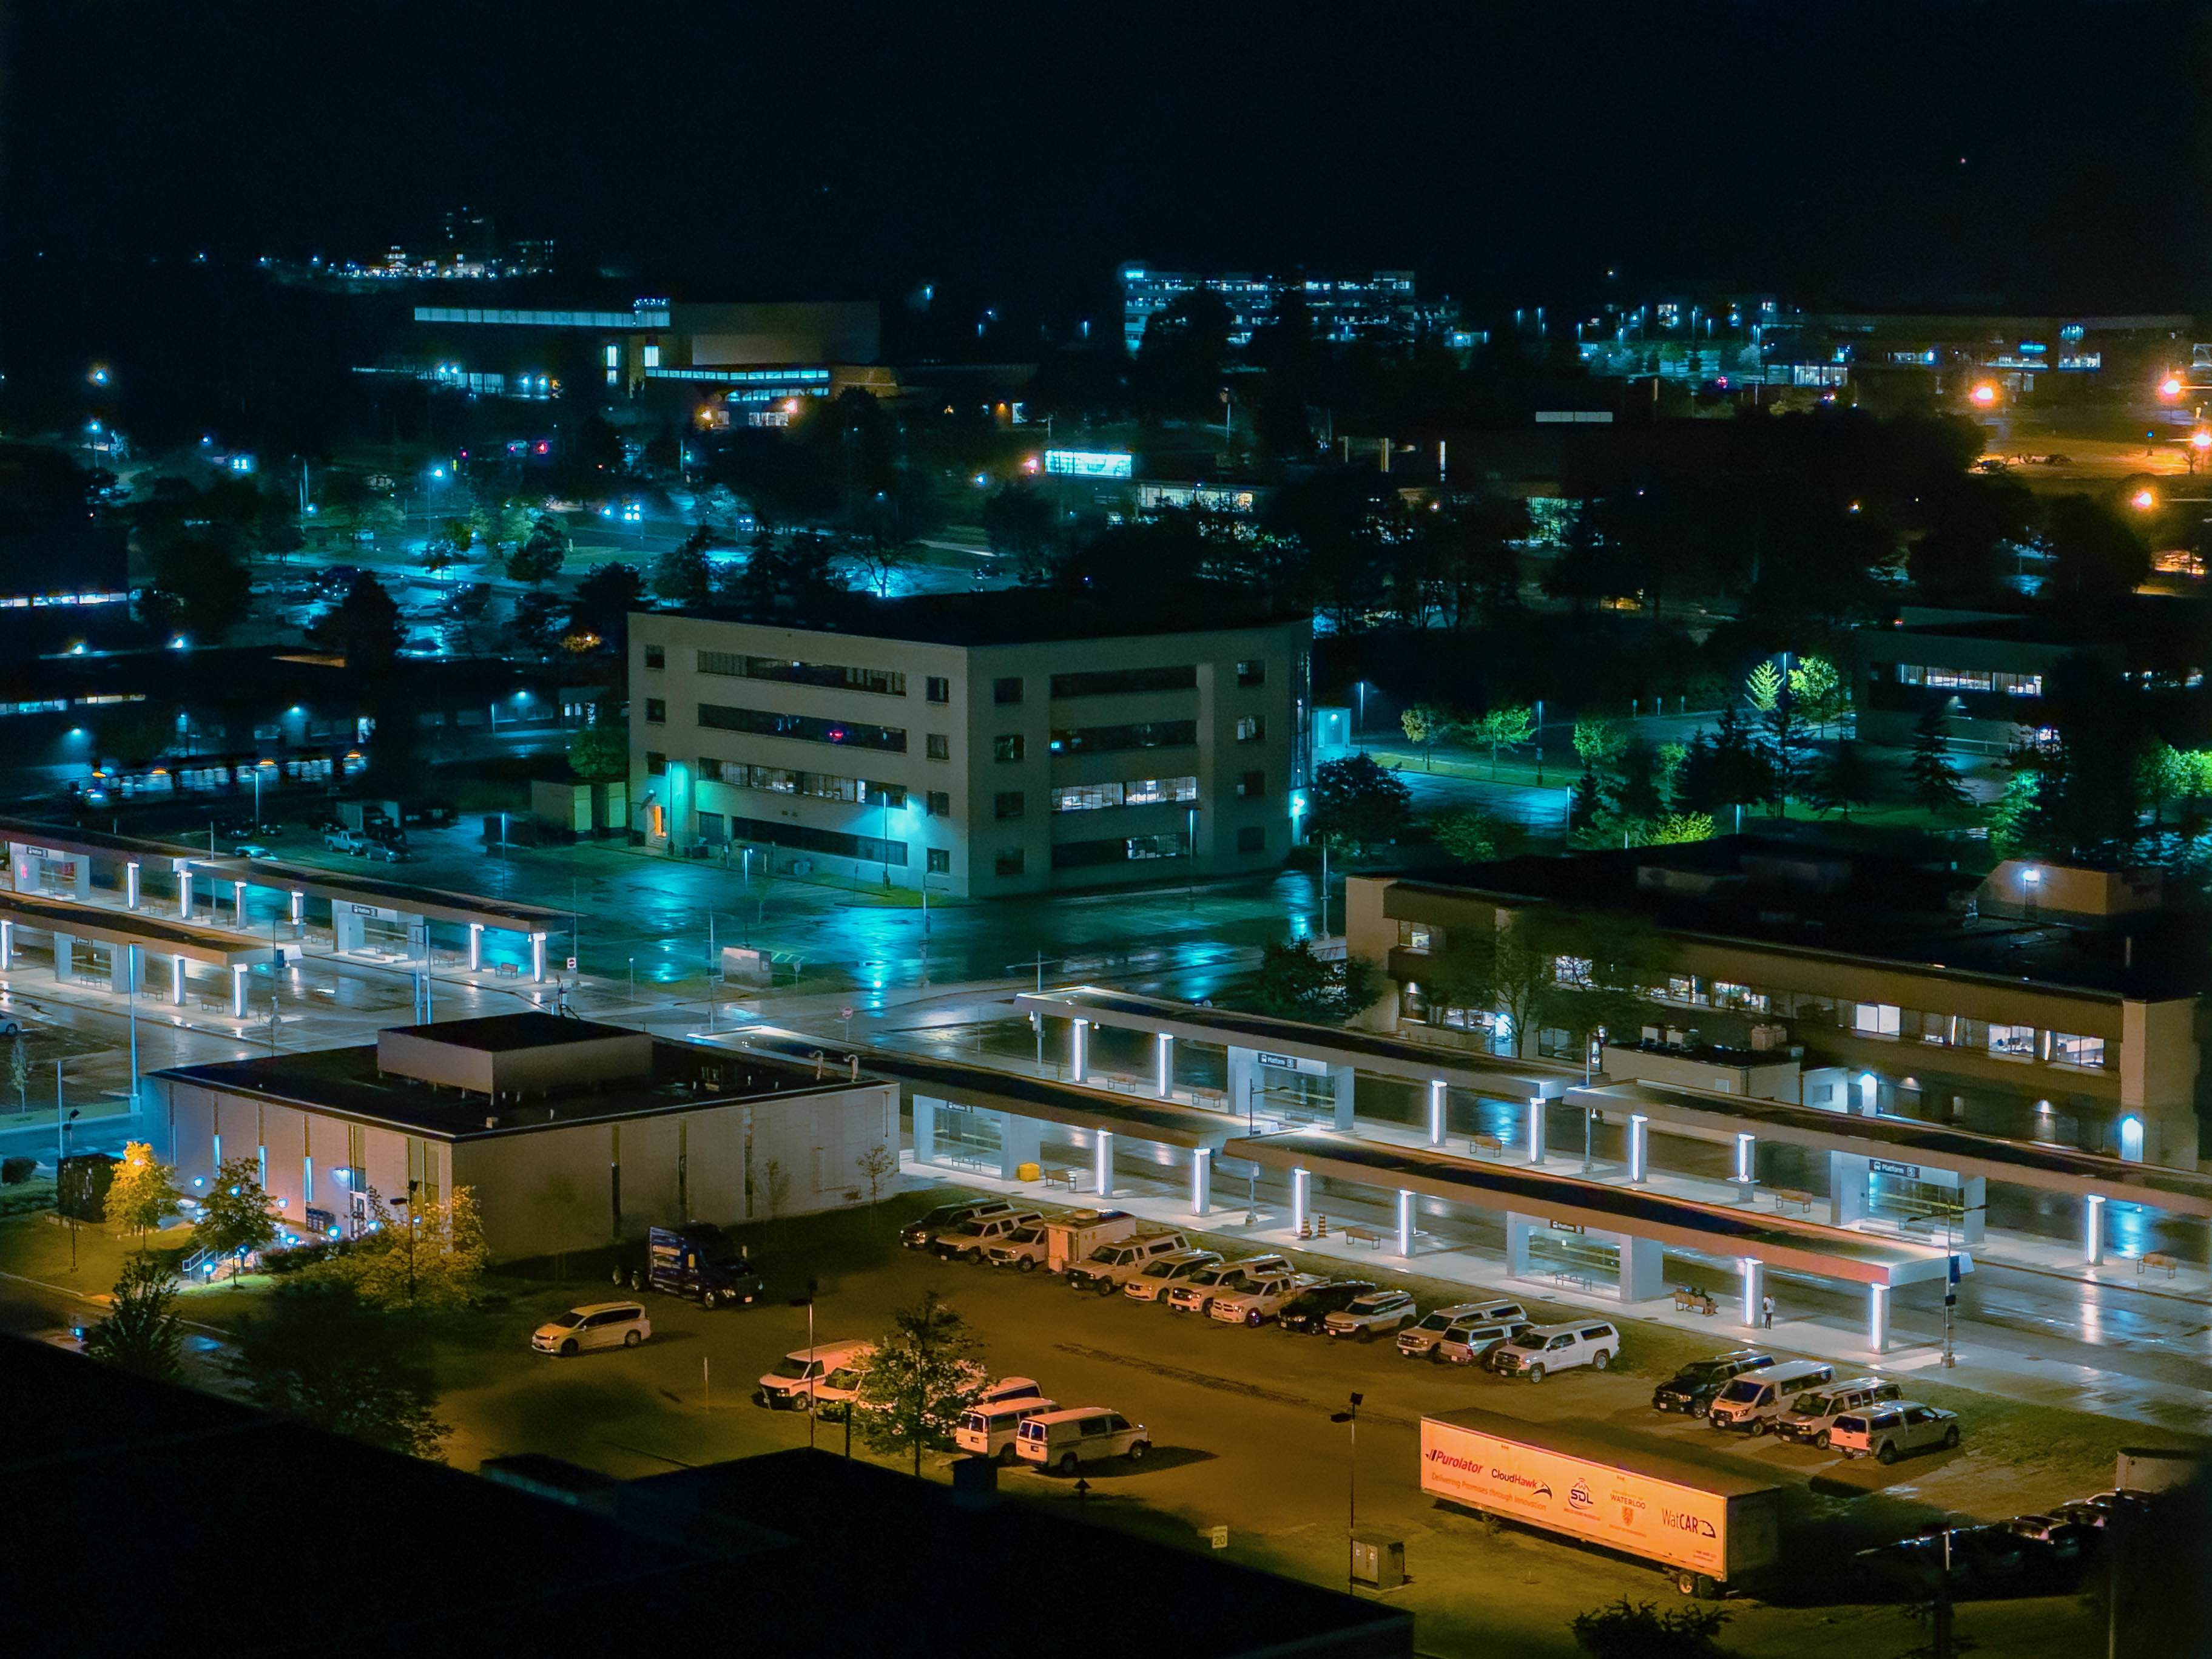
\includegraphics[scale=0.1]{loo.jpg}
    \caption{Waterloo, ON}
\end{figure}

\end{document}
